\documentclass[11pt,a4paper]{article}

\usepackage[margin=1in, paperwidth=8.3in, paperheight=11.7in]{geometry}
\usepackage{amsfonts}
\usepackage{amsmath}
\usepackage{enumerate}
\usepackage{enumitem}
\usepackage{fancyhdr}
\usepackage{stmaryrd}

\usepackage{tikz}
\usetikzlibrary{automata,positioning}

\begin{document}

\pagestyle{fancy}
\setlength\parindent{0pt}
\allowdisplaybreaks

% Counters
\newcounter{question}
\newcounter{qpart}[question]

% commands
\newcommand{\nats}{\mathbb{N}}
\newcommand{\real}{\mathbb{R}}
\newcommand{\newquestion} {\stepcounter{question}}
\newcommand{\newqpart} {\stepcounter{qpart}}
\newcommand{\question}[1] {\newquestion \ifquestions \textbf{Question \arabic{question}}\\ #1\\ \fi}
\newcommand{\Question}[1] {\newquestion \ifquestions \textbf{Question \arabic{question}}\\ #1 \fi}
\newcommand{\Qpart}[1] {\newquestion\newqpart \ifquestions \textbf{Question \arabic{question}.\arabic{qpart}}\\ #1\\ \fi}
\newcommand{\qpart}[1] {\newqpart \ifquestions \textbf{Question \arabic{question}.\arabic{qpart}}\\ #1\\ \fi}
\newcommand{\solution}[1] {\ifsolutions\textbf{My Solution \arabic{question}}\\ #1\\ \fi}
\newcommand{\Spart}[1] {\newqpart\ifsolutions\textbf{My Solution \arabic{question}.\arabic{qpart}}\\ #1\\ \fi}
\newcommand{\spart}[1] {\ifsolutions\textbf{My Solution \arabic{question}.\arabic{qpart}}\\ #1\\ \fi}
\newcommand{\doubleplus} {+\kern-1.3ex+\kern0.8ex}
\renewcommand{\headrulewidth}{0pt}

% if
\newif\ifquestions
\questionstrue
%\questionsfalse
\newif\ifsolutions
\solutionstrue
%\solutionsfalse

% Cover page title
\title{Data Structures \& Algorithms - Problem Sheet 3}
\author{Dom Hutchinson}
\date{\today}
\maketitle

% Header
\fancyhead[L]{Dom Hutchinson}
\fancyhead[C]{Data Structures \& Algorithms - Problem Sheet 3}
\fancyhead[R]{\today}

\question{
How many simple directed (unweighted) graphs on the set of vertices $\{v_1,v_2,\dots,v_n\}$ are there that have at most one edge between any pair of vertices?
(That is, for two vertices, $a\ \& b$, only at most one of the edges $(a,b)$ and $(b,a)$ is in the graph.) For this question vertices are distinct and isomorphic graphs are not the same (Graphs that have the same number of vertices and identical connections are said to be isomorphic). Justify your answer.
}

\solution{
There are $\frac{1}{2}n(n-1)$ unique pairs.\\
Each pair $(a,b)$ can be in one of three states: no edges; edge $a\to b$; or, edge $b\to a$.\\
Since each pair is independent this gives $\frac{3}{2}n(n-1)$ possible combinations.
}

\Question{
Given the visited node order for each of DFS and BFS starting with $s$, given the following adjancecy list
\begin{itemize}
  \item[] $s\to a,c,d$.
  \item[] $c\to e,b$.
  \item[] $b\to d$.
  \item[] $d\to c$.
  \item[] $e\to s$.
\end{itemize}
This can be visualised as\\
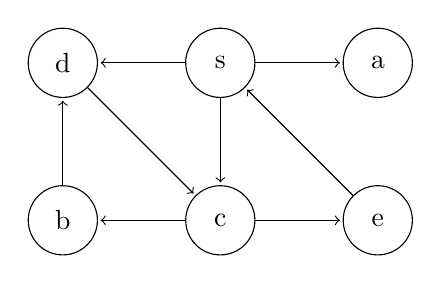
\begin{tikzpicture}[shorten >=1pt,node distance=2cm,on grid,auto]
   \node[state] (s)   {s};
   \node[state] (d) [left of= s] {d};
   \node[state] (a) [right of= s] {a};
   \node[state] (c) [below of= s] {c};
   \node[state] (b) [left of= c] {b};
   \node[state] (e) [right of= c] {e};
    \path[->]
    (s) edge node {} (a)
        edge node {} (c)
        edge node {} (d)
    (c) edge node {} (e)
        edge node {} (b)
    (b) edge node {} (d)
    (d) edge node {} (c)
    (e) edge node {} (s);
\end{tikzpicture}
}

\solution{
\textbf{DFS}\\
Let the leftmost element represent the top of the stack.\\
\begin{tabular}{|r|c|l|}
\hline
\# & Visit & Stack\\
\hline
i) & s & (acd)\\
ii)&a&(cd)\\
iii)&c&(ebd)\\
iv)&e&(sbd)\\
&s&(bd)\\
v)&b&(dd)\\
vi)&d&(d)\\
&d&()\\
\hline
\end{tabular}\\
In a depth first search the nodes are visited $s\to a\to c\to e\to b\to d$.\\

\textbf{BFS}\\
Consider elements to be push into the left of the queue, and popped off the right.\\
\begin{tabular}{|r|c|r|}
\hline
\# & Visit & Stack\\
\hline
i)&s&(dca)\\
ii)&a&(dc)\\
iii)&c&(bed)\\
iv)&d&(cbe)\\
v)&e&(scb)\\
vi)&b&(dsc)\\
&c&(ds)\\
&s&(d)\\
&d&()\\
\hline
\end{tabular}\\
In a breadth first search the nodes are visited $s\to a\to c\to b\to e\to d$.
}

\Qpart{
Is it true that both DFS and BFS require $\omega(|V|)$ storage for their operation?
}

\spart{
Yes, since you always have to store where you have been, which is $|V|$ nodes and in the best case you only ever have one node in the stack/queue.
}

\qpart{
How much storage do DFS and BFS require to visit all nodes of a tree starting at the root?
}

\spart{
\textbf{DFS}=$max(height)$.\\
\textbf{BFS}=$max(width)$.%NOTE not sure
}

\question{
In the Following graphs, assume that if there is ever a choice amongst multiple nodes, both the BFS \& DFS algorithms will choose the left-most node first. Starting from $S$ at the top, which algorithm will visit the least number of nodes before visiting $E$?
}

\qpart{
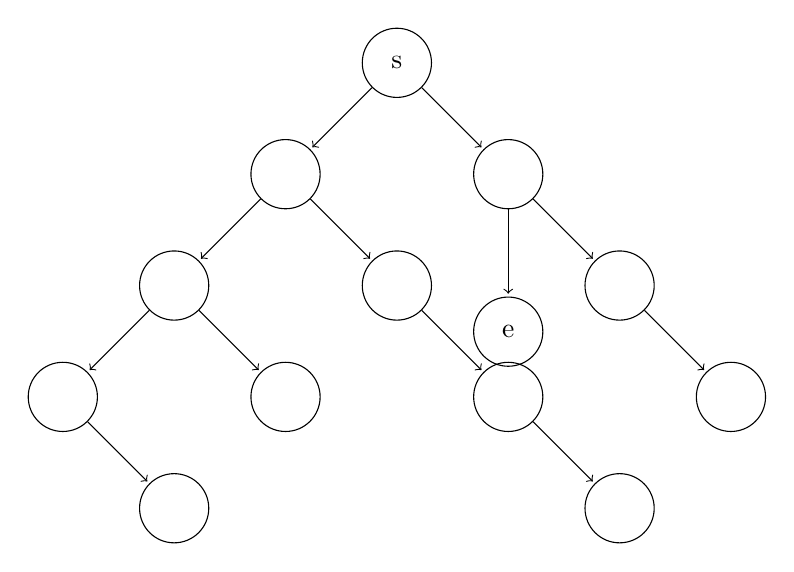
\begin{tikzpicture}[shorten >=1pt,node distance=2cm,on grid,auto]
   \node[state] (s) {s};
   \node[state] (1) [below left of= s] {};
   \node[state] (2) [below right of= s] {};
   \node[state] (3) [below left of= 1] {};
   \node[state] (4) [below right of= 1] {};
   \node[state] (e) [below of= 2] {e};
   \node[state] (5) [below right of= 2] {};
   \node[state] (6) [below left of= 3] {};
   \node[state] (7) [below right of= 3] {};
   \node[state] (8) [below right of= 4] {};
   \node[state] (9) [below right of= 5] {};
   \node[state] (10) [below right of= 6] {};
   \node[state] (11) [below right of= 8] {};
    \path[->]
    (s) edge node {} (1)
        edge node {} (2)
    (1) edge node {} (3)
        edge node {} (4)
    (2) edge node {} (e)
        edge node {} (5)
    (3) edge node {} (6)
        edge node {} (7)
    (4) edge node {} (8)
    (5) edge node {} (9)
    (6) edge node {} (10)
    (8) edge node {} (11);
\end{tikzpicture}
}

\spart{
\textbf{BFS}\\
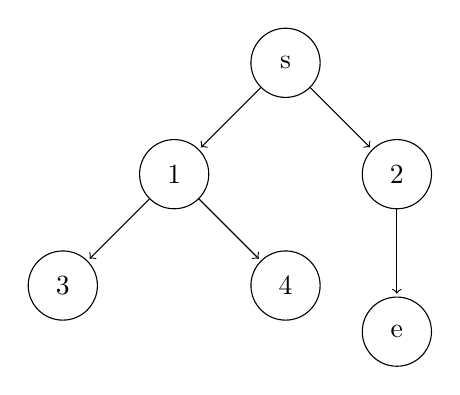
\begin{tikzpicture}[shorten >=1pt,node distance=2cm,on grid,auto]
   \node[state] (s) {s};
   \node[state] (1) [below left of= s] {1};
   \node[state] (2) [below right of= s] {2};
   \node[state] (3) [below left of= 1] {3};
   \node[state] (4) [below right of= 1] {4};
   \node[state] (e) [below of= 2] {e};
    \path[->]
    (s) edge node {} (1)
        edge node {} (2)
    (1) edge node {} (3)
        edge node {} (4)
    (2) edge node {} (e);
\end{tikzpicture}\\
In a breadth first search the nodes are met in the order shown above. So $e$ is met after $5$ nodes have been checked.\\

\textbf{DFS}\\
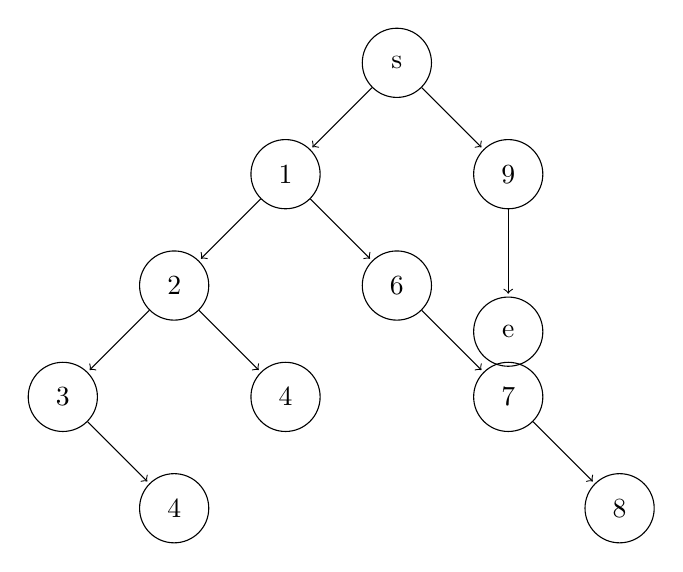
\begin{tikzpicture}[shorten >=1pt,node distance=2cm,on grid,auto]
   \node[state] (s) {s};
   \node[state] (1) [below left of= s] {1};
   \node[state] (2) [below right of= s] {9};
   \node[state] (3) [below left of= 1] {2};
   \node[state] (4) [below right of= 1] {6};
   \node[state] (e) [below of= 2] {e};
   \node[state] (6) [below left of= 3] {3};
   \node[state] (7) [below right of= 3] {4};
   \node[state] (8) [below right of= 4] {7};
   \node[state] (10) [below right of= 6] {4};
   \node[state] (11) [below right of= 8] {8};
    \path[->]
    (s) edge node {} (1)
        edge node {} (2)
    (1) edge node {} (3)
        edge node {} (4)
    (2) edge node {} (e)
    (3) edge node {} (6)
        edge node {} (7)
    (4) edge node {} (8)
    (6) edge node {} (10)
    (8) edge node {} (11);
\end{tikzpicture}\\
In a depth first search the nodes are met in the order shown above. So $e$ is met after $10$ nodes have been checked.\\
Thus \underline{BFS} meets $e$ quicker.
}

\qpart{
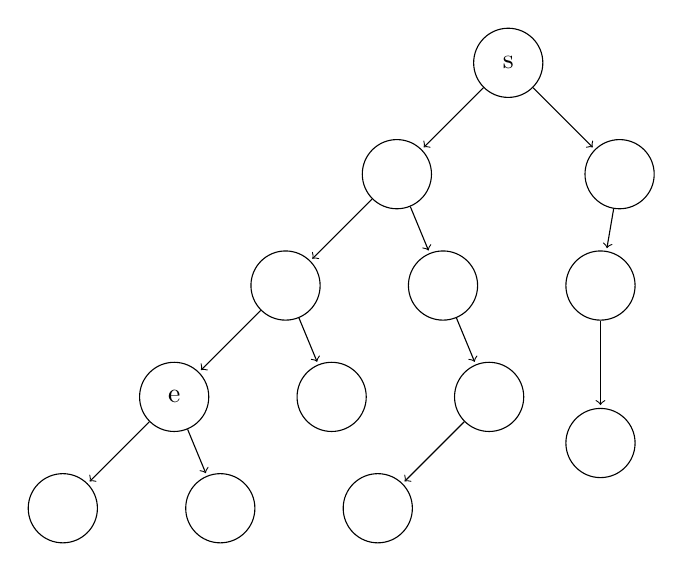
\begin{tikzpicture}[shorten >=1pt,node distance=2cm,on grid,auto]
   \node[state] (s) {s};
   \node[state] (1) [below left of= s] {};
   \node[state] (2) [below right of= s] {};
   \node[state] (3) [below left of= 1] {};
   \node[state] (4) [right of= 3] {};
   \node[state] (5) [right of= 4] {};
   \node[state] (e) [below left of= 3] {e};
   \node[state] (6) [right of= e] {};
   \node[state] (7) [right of= 6] {};
   \node[state] (8) [below of= 5] {};
   \node[state] (9) [below left of= e] {};
   \node[state] (10) [right of= 9] {};
   \node[state] (11) [below left of= 7] {};
    \path[->]
    (s) edge node {} (1)
        edge node {} (2)
    (1) edge node {} (3)
        edge node {} (4)
    (2) edge node {} (5)
    (3) edge node {} (e)
        edge node {} (6)
    (4) edge node {} (7)
    (5) edge node {} (8)
    (e) edge node {} (9)
        edge node {} (10)
    (7) edge node {} (11);
\end{tikzpicture}
}

\spart{
\textbf{BFS}\\
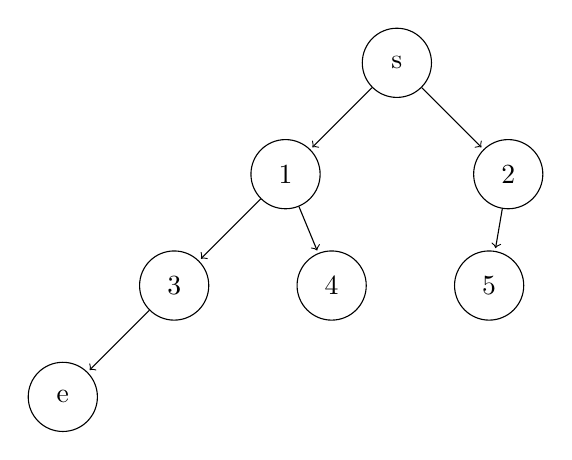
\begin{tikzpicture}[shorten >=1pt,node distance=2cm,on grid,auto]
   \node[state] (s) {s};
   \node[state] (1) [below left of= s] {1};
   \node[state] (2) [below right of= s] {2};
   \node[state] (3) [below left of= 1] {3};
   \node[state] (4) [right of= 3] {4};
   \node[state] (5) [right of= 4] {5};
   \node[state] (e) [below left of= 3] {e};
    \path[->]
    (s) edge node {} (1)
        edge node {} (2)
    (1) edge node {} (3)
        edge node {} (4)
    (2) edge node {} (5)
    (3) edge node {} (e);
\end{tikzpicture}\\
In a breadth first search the nodes are met in the order shown above. So $e$ is met after $5$ nodes have been checked.\\

\textbf{DFS}\\
\begin{tikzpicture}[shorten >=1pt,node distance=2cm,on grid,auto]
   \node[state] (s) {s};
   \node[state] (1) [below left of= s] {1};
   \node[state] (3) [below left of= 1] {2};
   \node[state] (e) [below left of= 3] {e};
    \path[->]
    (s) edge node {} (1)
    (1) edge node {} (3)
    (3) edge node {} (e);
\end{tikzpicture}\\
In a depth first search the nodes are met in the order shown above. So $e$ is met after $3$ nodes have been checked.\\
Thus \underline{DFS} meets $e$ quicker.
}

\question{
Given an example of a weighted graph $G$ for which BFS gives the incorrect shortest path between two nodes.
}

\solution{
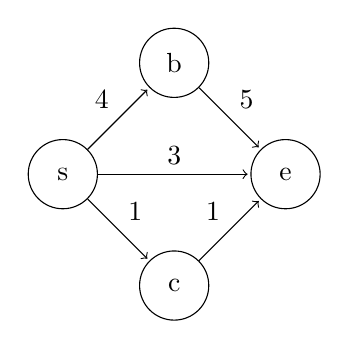
\begin{tikzpicture}[shorten >=1pt,node distance=2cm,on grid,auto]
   \node[state] (s) {s};
   \node[state] (b) [above right of= s] {b};
   \node[state] (c) [below right of= s] {c};
   \node[state] (e) [above right of= c] {e};
    \path[->]
    (s) edge node {4} (b)
        edge node {1} (c)
        edge node {3} (e)
    (b) edge node {5} (e)
    (c) edge node {1} (e);
\end{tikzpicture}\\
In this example a breadth first search would say the cheapest path from $s\to e$ costs $3$, when in fact going $s\to c\to e$ only costs $2$.
}

\Question{
What is the Discrete Fourier Transform of $1+2x+3x^2+4x^3$?
\begin{enumerate}[label=\roman*)]
  \item $5/2,\frac{-1+i}{2},-1/2,\frac{-1-i}{2}$
  \item $10,-2-2i,-2,-2+2i$
  \item$10,\frac{3-\sqrt{2}}{2}+\frac{2+\sqrt{2}}{2}i,3+\frac{\sqrt{2}}{2}+\frac{-2+\sqrt{2}}{2}i,-2,\frac{3+\sqrt{2}}{2}-\frac{-2+\sqrt{2}}{2}i,-2+2i,\frac{3+\sqrt{2}}{2}-\frac{2+\sqrt{2}}{2}i$
  \item$1,2,3,4$
  \item Something else
\end{enumerate}
}

\solution{
\[\begin{array}{rcl}
A(x)&=&1+2x+3x^2+4x^3\\
4^{th}\mathrm{\ Roots\ of\ Unity}&=&1,i,-1,-i\\

\\A(1)&=&1+2+3+4\\
&=&10\\
A(i)&=&1+2i-3-4i\\
&=&-2-2i\\
A(-1)&=&1-2+3-4\\
&=&2\\
A(-i)&=&1-2i-3+4i\\
&=&2i-2\\

\\y&=&(10,-2-2i,-2,2i-2)\\
&\equiv&\textbf{ii)}
\end{array}\]
}

\question{
Describe the generalisation of the FFT procedure to the case in which $n$ is a power of $3$.\\
Give the recurrence for the running time and solve the recurrence.
}

\Spart{
Define three polynomials
\[\begin{array}{rcl}
A^{[0]}&=&a_0+a_3x+\dots+a_{N-3}^{\frac{N}{3}-1}\\
A^{[1]}&=&a_1+a_4x+\dots+a_{N-2}^{\frac{N}{3}-1}\\
A^{[2]}&=&a_2+a_5x+\dots+a_{N-1}^{\frac{N}{3}-1}
\end{array}\]
Then
$$A(x)=A^{[0]}(x^3)+xA^{[1]}(x^3)+x^2A^{[2]}(x^3)$$
Evaluate $A(x)$ at $(\omega_N^0)^3,(\omega_N^1)^3,\dots, (\omega_N^{N-1})^3$.\\
Since $N$ is a power of $3$ we can use the cancellation lemma to show
$$(\omega_N^m)^3=\omega_N^3m=\omega_{N/3}^m\quad\forall\ m\in\nats_0$$
So there are a third as many complex roots of unity.\\
}

\Spart{
This process has a recurrence equation
\[\begin{array}{rrcl}
&T(1)&=&1\\
&T(n)&=&3T(\frac{n}{3})+\alpha n\quad\alpha\in\real\\

\\&T(n)&=&9T(\frac{n}{9})+2\alpha n\\
&&\vdots&\\
&&=&3^mT(\frac{n}{3^m})+\alpha mn\\
\mathrm{Until}&\frac{n}{3^m}&=&1\\
\implies&m&=&\log_3n\\
\implies&T(n)&=&3^{\log_3n}T(1)+\alpha n\log_3n\\
&&=&n.1+\alpha n\log_3n\\
&&=&\underline{n(1+\alpha\log_3n)}\in O(n\log_3 n)
\end{array}\]
}

\end{document}
